\documentclass{beamer}
\usetheme{Boadilla}

\usepackage{tikz}
\usepackage{proof}
\usepackage{amsmath, amsthm, amssymb}

\newtheorem{thm}{Theorem}
\newtheorem{lem}{Lemma}
\newtheorem{cor}{Corollary}
\newtheorem{defn}{Definition}

\newcommand{\2}{\textbf{2}}
\newcommand{\A}{\mathcal{A}}
\newcommand{\G}{\mathcal{G}}
\newcommand{\Z}{\mathbb{Z}}
\newcommand{\N}{\mathbb{N}}
\newcommand{\Q}{\mathbb{Q}}
\newcommand{\p}{\mathfrak{A}}
\newcommand{\del}{\partial}
\newcommand{\Am}{\textbf{A}}
\newcommand{\e}{\bar{e}}
\renewcommand{\r}{\bar{r}}
\renewcommand{\v}{\bar{v}}
\newcommand{\C}{\mathfrak{C}(\Am,\e)}

\title{Extensions of Abelian Automaton Groups}
\author{Chris Grossack\\ (Advisor: Klaus Sutner)}

\begin{document}

\begin{frame}
\titlepage%
\end{frame}

\begin{frame}{Let's Unpack That}
  \begin{center}
    \structure<2>{Extensions} of \structure<3>{Abelian} 
    \structure<4>{Automaton} \structure<5>{Groups}
  \end{center}
\end{frame}

\begin{frame}
  \tableofcontents%
\end{frame}

\section{Automata}
\begin{frame}{Finite State Automata}
  \begin{itemize}
    \item Combinatorial Objects
    \item Encode length preserving functions on binary strings
      \begin{itemize}
        \item states
        \item transitions
      \end{itemize}
  \end{itemize}

  \bigskip

  \begin{center}
  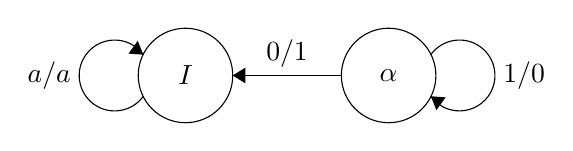
\begin{tikzpicture}[scale=0.2]
  \tikzstyle{every node}+=[inner sep=0pt]
  \draw [black] (23.2,-25.8) circle (3);
  \draw (23.2,-25.8) node {$I$};
  \draw [black] (36.1,-25.8) circle (3);
  \draw (36.1,-25.8) node {$\alpha$};
  \draw [black] (20.52,-27.123) arc (324:36:2.25);
  \draw (15.95,-25.8) node [left] {$a/a$};
  \fill [black] (20.52,-24.48) -- (20.17,-23.6) -- (19.58,-24.41);
  \draw [black] (33.1,-25.8) -- (26.2,-25.8);
  \fill [black] (26.2,-25.8) -- (27,-26.3) -- (27,-25.3);
  \draw (29.65,-25.3) node [above] {$0/1$};
  \draw [black] (38.78,-24.477) arc (144:-144:2.25);
  \draw (43.35,-25.8) node [right] {$1/0$};
  \fill [black] (38.78,-27.12) -- (39.13,-28) -- (39.72,-27.19);
  \end{tikzpicture}
  \end{center}

  \bigskip

  \begin{itemize}
    \item One function per state
    \item Evaluate by following edges
  \end{itemize}
\end{frame}

\begin{frame}{Evaluating Functions}
  \begin{itemize}
    \item $\mathcal{A}^3_2$. This automaton will be our friend 
      for the rest of this talk
    \item Defines three functions:
      \begin{itemize}
        \item $f$
        \item $f_0$
        \item $f_1$
      \end{itemize}
  \end{itemize}

  \bigskip

  \begin{center}
  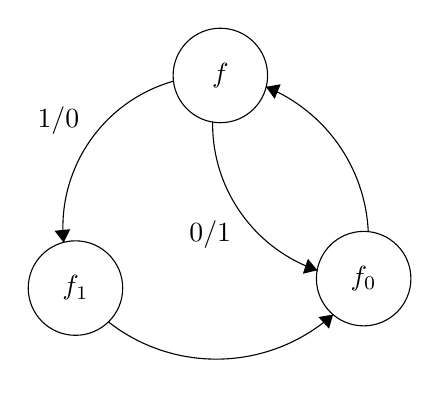
\begin{tikzpicture}[scale=0.2]
  \tikzstyle{every node}+=[inner sep=0pt]
  \draw [black] (26.6,-12.1) circle (3);
  \draw (26.6,-12.1) node {$f$};
  \draw [black] (17.4,-25.6) circle (3);
  \draw (17.4,-25.6) node {$f_1$};
  \draw [black] (35.7,-25) circle (3);
  \draw (35.7,-25) node {$f_0$};
  \draw [black] (16.648,-22.708) arc (-174.31762:-254.2298:9.658);
  \fill [black] (16.65,-22.71) -- (17.07,-21.86) -- (16.07,-21.96);
  \draw (17.67,-14.97) node [left] {$1/0$};
  \draw [black] (33.761,-27.277) arc (-48.14861:-128.09563:11.117);
  \fill [black] (33.76,-27.28) -- (32.83,-27.44) -- (33.5,-28.18);
  \draw [black] (29.501,-12.822) arc (67.8011:2.5992:10.451);
  \fill [black] (29.5,-12.82) -- (30.05,-13.59) -- (30.43,-12.66);
  \draw [black] (32.758,-24.474) arc (-108.88288:-180.71682:9.832);
  \fill [black] (32.76,-24.47) -- (32.16,-23.74) -- (31.84,-24.69);
  \draw (27.31,-22.21) node [left] {$0/1$};
  \end{tikzpicture}
  \end{center}

  \pause

  \begin{itemize}
    \item How do we compute, say, $f$ of a string?
  \end{itemize}
  
\end{frame}

\begin{frame}{Evaluating Functions}
  \begin{center}
  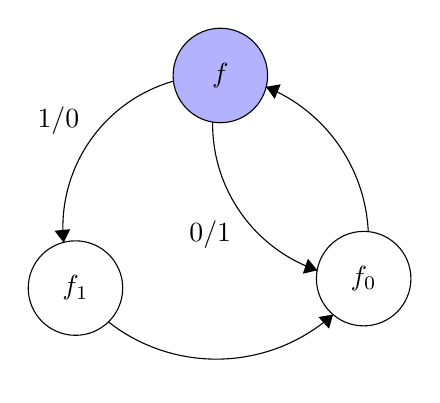
\begin{tikzpicture}[scale=0.2]
  \tikzstyle{every node}+=[inner sep=0pt]
  \draw [black, fill=blue!30] (26.6,-12.1) circle (3);
  \draw (26.6,-12.1) node {$f$};
  \draw [black] (17.4,-25.6) circle (3);
  \draw (17.4,-25.6) node {$f_1$};
  \draw [black] (35.7,-25) circle (3);
  \draw (35.7,-25) node {$f_0$};
  \draw [black] (16.648,-22.708) arc (-174.31762:-254.2298:9.658);
  \fill [black] (16.65,-22.71) -- (17.07,-21.86) -- (16.07,-21.96);
  \draw (17.67,-14.97) node [left] {$1/0$};
  \draw [black] (33.761,-27.277) arc (-48.14861:-128.09563:11.117);
  \fill [black] (33.76,-27.28) -- (32.83,-27.44) -- (33.5,-28.18);
  \draw [black] (29.501,-12.822) arc (67.8011:2.5992:10.451);
  \fill [black] (29.5,-12.82) -- (30.05,-13.59) -- (30.43,-12.66);
  \draw [black] (32.758,-24.474) arc (-108.88288:-180.71682:9.832);
  \fill [black] (32.76,-24.47) -- (32.16,-23.74) -- (31.84,-24.69);
  \draw (27.31,-22.21) node [left] {$0/1$};
  \end{tikzpicture}
  \end{center}
  
  \bigskip

  \begin{itemize}
    \item $f(011010)$
  \end{itemize}
\end{frame}

\begin{frame}{Evaluating Functions}
  \begin{center}
  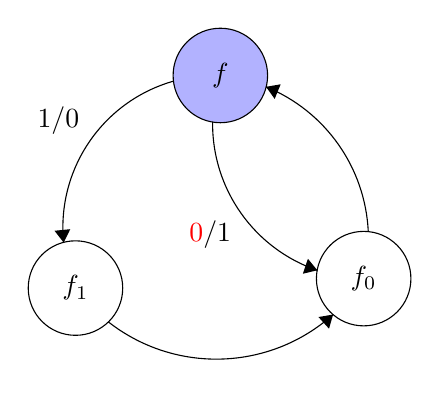
\begin{tikzpicture}[scale=0.2]
  \tikzstyle{every node}+=[inner sep=0pt]
  \draw [black, fill=blue!30] (26.6,-12.1) circle (3);
  \draw (26.6,-12.1) node {$f$};
  \draw [black] (17.4,-25.6) circle (3);
  \draw (17.4,-25.6) node {$f_1$};
  \draw [black] (35.7,-25) circle (3);
  \draw (35.7,-25) node {$f_0$};
  \draw [black] (16.648,-22.708) arc (-174.31762:-254.2298:9.658);
  \fill [black] (16.65,-22.71) -- (17.07,-21.86) -- (16.07,-21.96);
  \draw (17.67,-14.97) node [left] {$1/0$};
  \draw [black] (33.761,-27.277) arc (-48.14861:-128.09563:11.117);
  \fill [black] (33.76,-27.28) -- (32.83,-27.44) -- (33.5,-28.18);
  \draw [black] (29.501,-12.822) arc (67.8011:2.5992:10.451);
  \fill [black] (29.5,-12.82) -- (30.05,-13.59) -- (30.43,-12.66);
  \draw [black] (32.758,-24.474) arc (-108.88288:-180.71682:9.832);
  \fill [black] (32.76,-24.47) -- (32.16,-23.74) -- (31.84,-24.69);
    \draw (27.31,-22.21) node [left] {$\textcolor{red}{0}/1$};
  \end{tikzpicture}
  \end{center}
  
  \bigskip

  \begin{itemize}
    \item $f(\textcolor{red}011010)$
  \end{itemize}
\end{frame}

\begin{frame}{Evaluating Functions}
  \begin{center}
  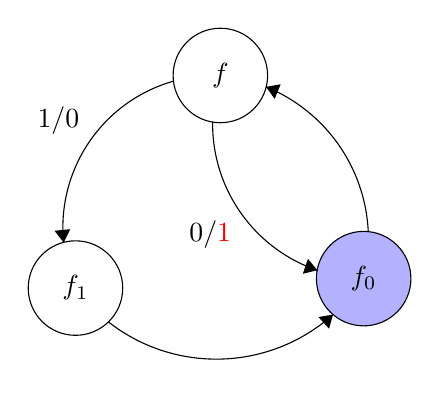
\begin{tikzpicture}[scale=0.2]
  \tikzstyle{every node}+=[inner sep=0pt]
  \draw [black] (26.6,-12.1) circle (3);
  \draw (26.6,-12.1) node {$f$};
  \draw [black] (17.4,-25.6) circle (3);
  \draw (17.4,-25.6) node {$f_1$};
  \draw [black, fill=blue!30] (35.7,-25) circle (3);
  \draw (35.7,-25) node {$f_0$};
  \draw [black] (16.648,-22.708) arc (-174.31762:-254.2298:9.658);
  \fill [black] (16.65,-22.71) -- (17.07,-21.86) -- (16.07,-21.96);
  \draw (17.67,-14.97) node [left] {$1/0$};
  \draw [black] (33.761,-27.277) arc (-48.14861:-128.09563:11.117);
  \fill [black] (33.76,-27.28) -- (32.83,-27.44) -- (33.5,-28.18);
  \draw [black] (29.501,-12.822) arc (67.8011:2.5992:10.451);
  \fill [black] (29.5,-12.82) -- (30.05,-13.59) -- (30.43,-12.66);
  \draw [black] (32.758,-24.474) arc (-108.88288:-180.71682:9.832);
  \fill [black] (32.76,-24.47) -- (32.16,-23.74) -- (31.84,-24.69);
    \draw (27.31,-22.21) node [left] {$0/\textcolor{red}{1}$};
  \end{tikzpicture}
  \end{center}
  
  \bigskip

  \begin{itemize}
    \item \textcolor{red}{1}$f_0(11010)$
  \end{itemize}
\end{frame}

\begin{frame}{Evaluating Functions}
  \begin{center}
  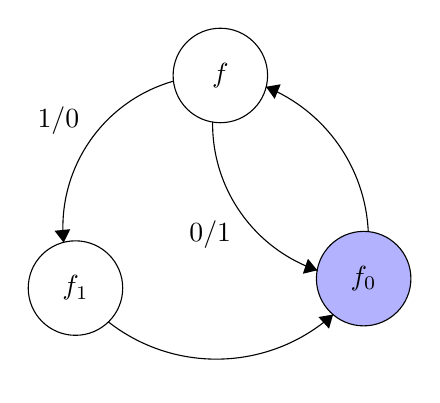
\begin{tikzpicture}[scale=0.2]
  \tikzstyle{every node}+=[inner sep=0pt]
  \draw [black] (26.6,-12.1) circle (3);
  \draw (26.6,-12.1) node {$f$};
  \draw [black] (17.4,-25.6) circle (3);
  \draw (17.4,-25.6) node {$f_1$};
  \draw [black, fill=blue!30] (35.7,-25) circle (3);
  \draw (35.7,-25) node {$f_0$};
  \draw [black] (16.648,-22.708) arc (-174.31762:-254.2298:9.658);
  \fill [black] (16.65,-22.71) -- (17.07,-21.86) -- (16.07,-21.96);
  \draw (17.67,-14.97) node [left] {$1/0$};
  \draw [black] (33.761,-27.277) arc (-48.14861:-128.09563:11.117);
  \fill [black] (33.76,-27.28) -- (32.83,-27.44) -- (33.5,-28.18);
  \draw [black] (29.501,-12.822) arc (67.8011:2.5992:10.451);
  \fill [black] (29.5,-12.82) -- (30.05,-13.59) -- (30.43,-12.66);
  \draw [black] (32.758,-24.474) arc (-108.88288:-180.71682:9.832);
  \fill [black] (32.76,-24.47) -- (32.16,-23.74) -- (31.84,-24.69);
  \draw (27.31,-22.21) node [left] {$0/1$};
  \end{tikzpicture}
  \end{center}
  
  \bigskip

  \begin{itemize}
    \item $1 f_0(11010)$
  \end{itemize}
\end{frame}

\begin{frame}{Evaluating Functions}
  \begin{center}
  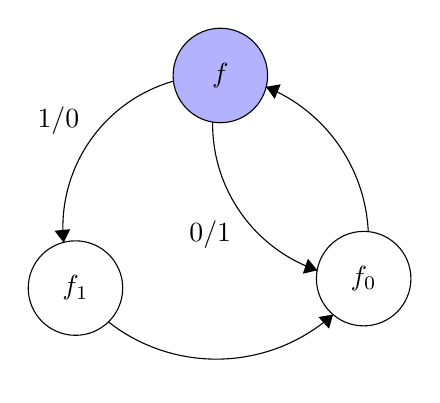
\begin{tikzpicture}[scale=0.2]
  \tikzstyle{every node}+=[inner sep=0pt]
  \draw [black, fill=blue!30] (26.6,-12.1) circle (3);
  \draw (26.6,-12.1) node {$f$};
  \draw [black] (17.4,-25.6) circle (3);
  \draw (17.4,-25.6) node {$f_1$};
  \draw [black] (35.7,-25) circle (3);
  \draw (35.7,-25) node {$f_0$};
  \draw [black] (16.648,-22.708) arc (-174.31762:-254.2298:9.658);
  \fill [black] (16.65,-22.71) -- (17.07,-21.86) -- (16.07,-21.96);
  \draw (17.67,-14.97) node [left] {$1/0$};
  \draw [black] (33.761,-27.277) arc (-48.14861:-128.09563:11.117);
  \fill [black] (33.76,-27.28) -- (32.83,-27.44) -- (33.5,-28.18);
  \draw [black] (29.501,-12.822) arc (67.8011:2.5992:10.451);
  \fill [black] (29.5,-12.82) -- (30.05,-13.59) -- (30.43,-12.66);
  \draw [black] (32.758,-24.474) arc (-108.88288:-180.71682:9.832);
  \fill [black] (32.76,-24.47) -- (32.16,-23.74) -- (31.84,-24.69);
  \draw (27.31,-22.21) node [left] {$0/1$};
  \end{tikzpicture}
  \end{center}
  
  \bigskip

  \begin{itemize}
    \item $11 f(1010)$
  \end{itemize}
\end{frame}

\begin{frame}{Evaluating Functions}
  \begin{center}
  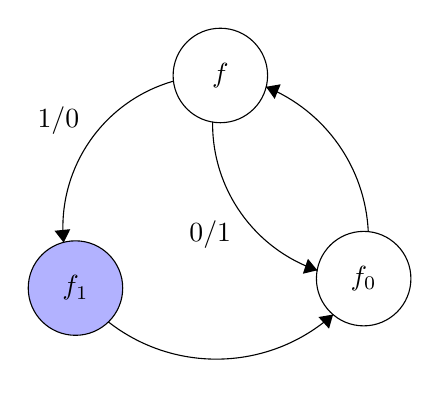
\begin{tikzpicture}[scale=0.2]
  \tikzstyle{every node}+=[inner sep=0pt]
  \draw [black] (26.6,-12.1) circle (3);
  \draw (26.6,-12.1) node {$f$};
  \draw [black, fill=blue!30] (17.4,-25.6) circle (3);
  \draw (17.4,-25.6) node {$f_1$};
  \draw [black] (35.7,-25) circle (3);
  \draw (35.7,-25) node {$f_0$};
  \draw [black] (16.648,-22.708) arc (-174.31762:-254.2298:9.658);
  \fill [black] (16.65,-22.71) -- (17.07,-21.86) -- (16.07,-21.96);
  \draw (17.67,-14.97) node [left] {$1/0$};
  \draw [black] (33.761,-27.277) arc (-48.14861:-128.09563:11.117);
  \fill [black] (33.76,-27.28) -- (32.83,-27.44) -- (33.5,-28.18);
  \draw [black] (29.501,-12.822) arc (67.8011:2.5992:10.451);
  \fill [black] (29.5,-12.82) -- (30.05,-13.59) -- (30.43,-12.66);
  \draw [black] (32.758,-24.474) arc (-108.88288:-180.71682:9.832);
  \fill [black] (32.76,-24.47) -- (32.16,-23.74) -- (31.84,-24.69);
  \draw (27.31,-22.21) node [left] {$0/1$};
  \end{tikzpicture}
  \end{center}
  
  \bigskip

  \begin{itemize}
    \item $110 f_1(010)$
  \end{itemize}
\end{frame}

\begin{frame}{Evaluating Functions}
  \begin{center}
  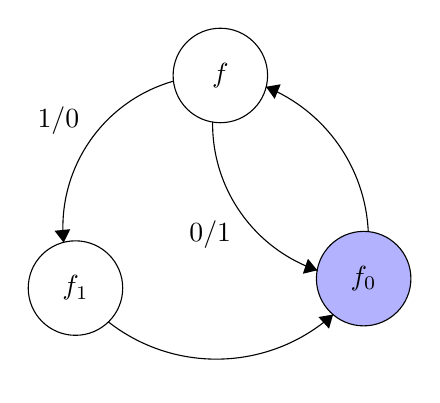
\begin{tikzpicture}[scale=0.2]
  \tikzstyle{every node}+=[inner sep=0pt]
  \draw [black] (26.6,-12.1) circle (3);
  \draw (26.6,-12.1) node {$f$};
  \draw [black] (17.4,-25.6) circle (3);
  \draw (17.4,-25.6) node {$f_1$};
  \draw [black, fill=blue!30] (35.7,-25) circle (3);
  \draw (35.7,-25) node {$f_0$};
  \draw [black] (16.648,-22.708) arc (-174.31762:-254.2298:9.658);
  \fill [black] (16.65,-22.71) -- (17.07,-21.86) -- (16.07,-21.96);
  \draw (17.67,-14.97) node [left] {$1/0$};
  \draw [black] (33.761,-27.277) arc (-48.14861:-128.09563:11.117);
  \fill [black] (33.76,-27.28) -- (32.83,-27.44) -- (33.5,-28.18);
  \draw [black] (29.501,-12.822) arc (67.8011:2.5992:10.451);
  \fill [black] (29.5,-12.82) -- (30.05,-13.59) -- (30.43,-12.66);
  \draw [black] (32.758,-24.474) arc (-108.88288:-180.71682:9.832);
  \fill [black] (32.76,-24.47) -- (32.16,-23.74) -- (31.84,-24.69);
  \draw (27.31,-22.21) node [left] {$0/1$};
  \end{tikzpicture}
  \end{center}
  
  \bigskip

  \begin{itemize}
    \item $1100 f_0(10)$
  \end{itemize}
\end{frame}

\begin{frame}{Evaluating Functions}
  \begin{center}
  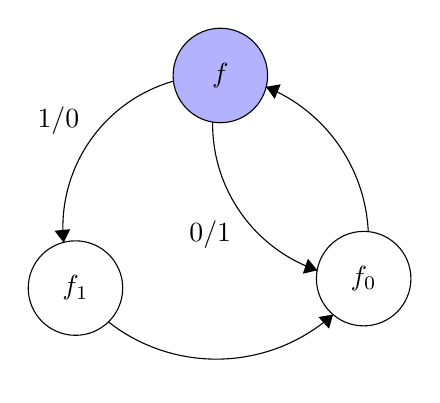
\begin{tikzpicture}[scale=0.2]
  \tikzstyle{every node}+=[inner sep=0pt]
  \draw [black, fill=blue!30] (26.6,-12.1) circle (3);
  \draw (26.6,-12.1) node {$f$};
  \draw [black] (17.4,-25.6) circle (3);
  \draw (17.4,-25.6) node {$f_1$};
  \draw [black] (35.7,-25) circle (3);
  \draw (35.7,-25) node {$f_0$};
  \draw [black] (16.648,-22.708) arc (-174.31762:-254.2298:9.658);
  \fill [black] (16.65,-22.71) -- (17.07,-21.86) -- (16.07,-21.96);
  \draw (17.67,-14.97) node [left] {$1/0$};
  \draw [black] (33.761,-27.277) arc (-48.14861:-128.09563:11.117);
  \fill [black] (33.76,-27.28) -- (32.83,-27.44) -- (33.5,-28.18);
  \draw [black] (29.501,-12.822) arc (67.8011:2.5992:10.451);
  \fill [black] (29.5,-12.82) -- (30.05,-13.59) -- (30.43,-12.66);
  \draw [black] (32.758,-24.474) arc (-108.88288:-180.71682:9.832);
  \fill [black] (32.76,-24.47) -- (32.16,-23.74) -- (31.84,-24.69);
  \draw (27.31,-22.21) node [left] {$0/1$};
  \end{tikzpicture}
  \end{center}
  
  \bigskip

  \begin{itemize}
    \item $11001 f(0)$
  \end{itemize}
\end{frame}

\begin{frame}{Evaluating Functions}
  \begin{center}
  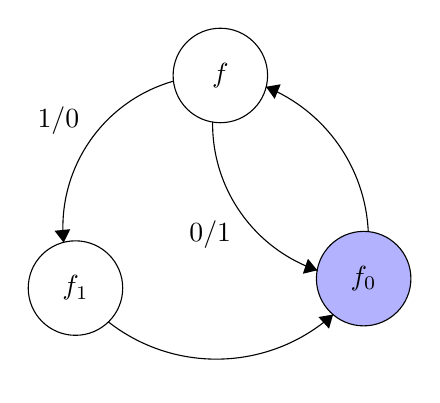
\begin{tikzpicture}[scale=0.2]
  \tikzstyle{every node}+=[inner sep=0pt]
  \draw [black] (26.6,-12.1) circle (3);
  \draw (26.6,-12.1) node {$f$};
  \draw [black] (17.4,-25.6) circle (3);
  \draw (17.4,-25.6) node {$f_1$};
  \draw [black, fill=blue!30] (35.7,-25) circle (3);
  \draw (35.7,-25) node {$f_0$};
  \draw [black] (16.648,-22.708) arc (-174.31762:-254.2298:9.658);
  \fill [black] (16.65,-22.71) -- (17.07,-21.86) -- (16.07,-21.96);
  \draw (17.67,-14.97) node [left] {$1/0$};
  \draw [black] (33.761,-27.277) arc (-48.14861:-128.09563:11.117);
  \fill [black] (33.76,-27.28) -- (32.83,-27.44) -- (33.5,-28.18);
  \draw [black] (29.501,-12.822) arc (67.8011:2.5992:10.451);
  \fill [black] (29.5,-12.82) -- (30.05,-13.59) -- (30.43,-12.66);
  \draw [black] (32.758,-24.474) arc (-108.88288:-180.71682:9.832);
  \fill [black] (32.76,-24.47) -- (32.16,-23.74) -- (31.84,-24.69);
  \draw (27.31,-22.21) node [left] {$0/1$};
  \end{tikzpicture}
  \end{center}
  
  \bigskip

  \begin{itemize}
    \item $110011 f_0(\varepsilon)$
  \end{itemize}
\end{frame}

\begin{frame}{Evaluating Functions}
  \begin{center}
  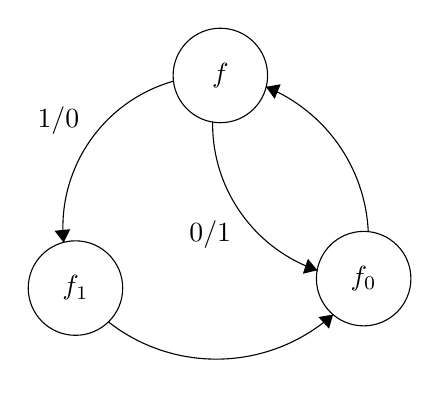
\begin{tikzpicture}[scale=0.2]
  \tikzstyle{every node}+=[inner sep=0pt]
  \draw [black] (26.6,-12.1) circle (3);
  \draw (26.6,-12.1) node {$f$};
  \draw [black] (17.4,-25.6) circle (3);
  \draw (17.4,-25.6) node {$f_1$};
  \draw [black] (35.7,-25) circle (3);
  \draw (35.7,-25) node {$f_0$};
  \draw [black] (16.648,-22.708) arc (-174.31762:-254.2298:9.658);
  \fill [black] (16.65,-22.71) -- (17.07,-21.86) -- (16.07,-21.96);
  \draw (17.67,-14.97) node [left] {$1/0$};
  \draw [black] (33.761,-27.277) arc (-48.14861:-128.09563:11.117);
  \fill [black] (33.76,-27.28) -- (32.83,-27.44) -- (33.5,-28.18);
  \draw [black] (29.501,-12.822) arc (67.8011:2.5992:10.451);
  \fill [black] (29.5,-12.82) -- (30.05,-13.59) -- (30.43,-12.66);
  \draw [black] (32.758,-24.474) arc (-108.88288:-180.71682:9.832);
  \fill [black] (32.76,-24.47) -- (32.16,-23.74) -- (31.84,-24.69);
  \draw (27.31,-22.21) node [left] {$0/1$};
  \end{tikzpicture}
  \end{center}
  
  \bigskip

  \begin{itemize}
    \item $110011$
  \end{itemize}
\end{frame}

\begin{frame}
  \begin{defn}
    $\del_0 f$ (resp. $\del_1 f$) is the unique function such that
    for every $w \in 2^*$, $f(0w) = (f(0)) (\del_0 f)(w)$
  \end{defn}

  \pause

  \begin{defn}
    A state $f$ is called \structure{Odd} if it flips its input bit, and 
    \structure{Even} otherwise.
  \end{defn}

  \pause

  \begin{center}
  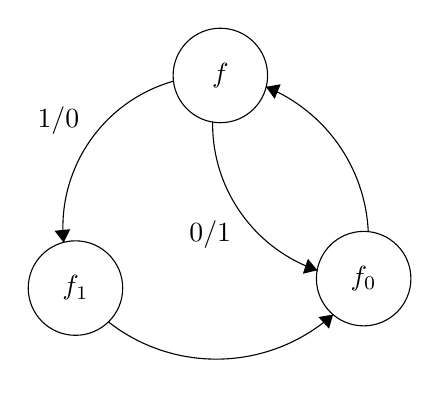
\begin{tikzpicture}[scale=0.2]
  \tikzstyle{every node}+=[inner sep=0pt]
  \draw [black] (26.6,-12.1) circle (3);
  \draw (26.6,-12.1) node {$f$};
  \draw [black] (17.4,-25.6) circle (3);
  \draw (17.4,-25.6) node {$f_1$};
  \draw [black] (35.7,-25) circle (3);
  \draw (35.7,-25) node {$f_0$};
  \draw [black] (16.648,-22.708) arc (-174.31762:-254.2298:9.658);
  \fill [black] (16.65,-22.71) -- (17.07,-21.86) -- (16.07,-21.96);
  \draw (17.67,-14.97) node [left] {$1/0$};
  \draw [black] (33.761,-27.277) arc (-48.14861:-128.09563:11.117);
  \fill [black] (33.76,-27.28) -- (32.83,-27.44) -- (33.5,-28.18);
  \draw [black] (29.501,-12.822) arc (67.8011:2.5992:10.451);
  \fill [black] (29.5,-12.82) -- (30.05,-13.59) -- (30.43,-12.66);
  \draw [black] (32.758,-24.474) arc (-108.88288:-180.71682:9.832);
  \fill [black] (32.76,-24.47) -- (32.16,-23.74) -- (31.84,-24.69);
  \draw (27.31,-22.21) node [left] {$0/1$};
  \end{tikzpicture}
  \end{center}

  \begin{itemize}
    \item $\del_0 f = f_0$ and $\del_1 f = f_1$
    \item $f$ is odd, $f_0$ and $f_1$ are even
  \end{itemize}
\end{frame}

\section{Abelian}
\begin{frame}
  \begin{defn}
    For $f$ and $g$ in an automaton $\A$, write $f+g$ for the function
    $(f+g)(x) = f(g(x))$
  \end{defn}

  \pause

  \begin{itemize}
    \item We are interested in the \structure{Abelian} case.
    \pause
    \item For all of our machines, $f+g = g+f$
    \pause
    \item Given a machine $\A$, this condition is checkable in polynomial time
  \end{itemize}
\end{frame}

\section{Groups}
\begin{frame}
  \begin{defn}
    Recall a \structure{Group} is a set $\G$ equipped with
    \begin{itemize}
      \item $0 \in \G$
      \item $+ : \G \to \G \to \G$ (associative)
      \item $- : \G \to \G$
      \item satisfying $0+x = x+0 = x$ and $x + (-x) = (-x) + x = 0$
    \end{itemize}
  \end{defn}
  
  \pause

  \begin{itemize}
    \item If $S$ is the state set of an automaton $\A$, consider 
      $\G$ to be the closure of $S$ under $+$ 
    \item take $0=id : 2^* \to 2^*$ to be the empty sum
    \pause
    \item This does not have $-$ in general
    \item Our functions don't even need to be \emph{invertible}
    \pause
    \item Each function is invertible iff each state is invertible in one step
  \end{itemize}
\end{frame}

\begin{frame}{The Inverse Automaton}
  \begin{itemize}
    \item Since each state sees an invertible function\ldots invert it.
  \end{itemize}
  \pause
  \bigskip
  \begin{columns}
    \column{0.5\textwidth}
    $\A^3_2$
    \begin{center}
    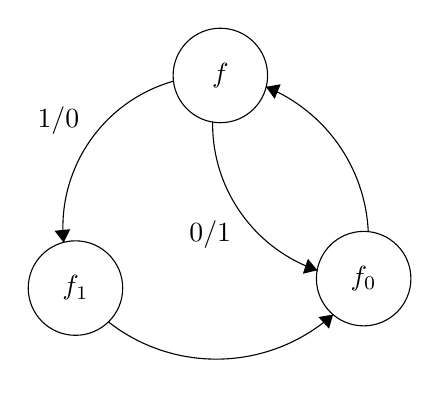
\begin{tikzpicture}[scale=0.2]
    \tikzstyle{every node}+=[inner sep=0pt]
    \draw [black] (26.6,-12.1) circle (3);
    \draw (26.6,-12.1) node {$f$};
    \draw [black] (17.4,-25.6) circle (3);
    \draw (17.4,-25.6) node {$f_1$};
    \draw [black] (35.7,-25) circle (3);
    \draw (35.7,-25) node {$f_0$};
    \draw [black] (16.648,-22.708) arc (-174.31762:-254.2298:9.658);
    \fill [black] (16.65,-22.71) -- (17.07,-21.86) -- (16.07,-21.96);
    \draw (17.67,-14.97) node [left] {$1/0$};
    \draw [black] (33.761,-27.277) arc (-48.14861:-128.09563:11.117);
    \fill [black] (33.76,-27.28) -- (32.83,-27.44) -- (33.5,-28.18);
    \draw [black] (29.501,-12.822) arc (67.8011:2.5992:10.451);
    \fill [black] (29.5,-12.82) -- (30.05,-13.59) -- (30.43,-12.66);
    \draw [black] (32.758,-24.474) arc (-108.88288:-180.71682:9.832);
    \fill [black] (32.76,-24.47) -- (32.16,-23.74) -- (31.84,-24.69);
    \draw (27.31,-22.21) node [left] {$0/1$};
    \end{tikzpicture}
    \end{center}

    \column{0.5\textwidth}
    $-\A^3_2$
    \begin{center}
    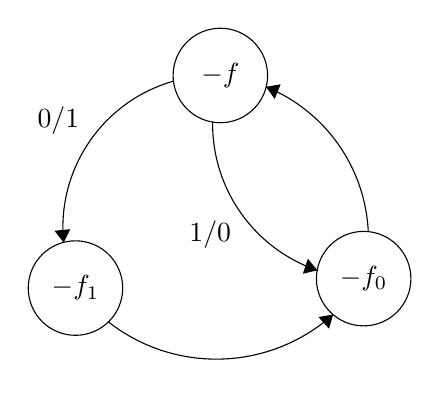
\begin{tikzpicture}[scale=0.2]
    \tikzstyle{every node}+=[inner sep=0pt]
    \draw [black] (26.6,-12.1) circle (3);
    \draw (26.6,-12.1) node {$-f$};
    \draw [black] (17.4,-25.6) circle (3);
    \draw (17.4,-25.6) node {$-f_1$};
    \draw [black] (35.7,-25) circle (3);
    \draw (35.7,-25) node {$-f_0$};
    \draw [black] (16.648,-22.708) arc (-174.31762:-254.2298:9.658);
    \fill [black] (16.65,-22.71) -- (17.07,-21.86) -- (16.07,-21.96);
    \draw (17.67,-14.97) node [left] {$0/1$};
    \draw [black] (33.761,-27.277) arc (-48.14861:-128.09563:11.117);
    \fill [black] (33.76,-27.28) -- (32.83,-27.44) -- (33.5,-28.18);
    \draw [black] (29.501,-12.822) arc (67.8011:2.5992:10.451);
    \fill [black] (29.5,-12.82) -- (30.05,-13.59) -- (30.43,-12.66);
    \draw [black] (32.758,-24.474) arc (-108.88288:-180.71682:9.832);
    \fill [black] (32.76,-24.47) -- (32.16,-23.74) -- (31.84,-24.69);
    \draw (27.31,-22.21) node [left] {$1/0$};
    \end{tikzpicture}
    \end{center}
  \end{columns}
  
  \pause

  \begin{itemize}
    \item Take Care: $\del_0 (-f) = -\del_1 f$
    \pause
    \item But: $(f + (-f))(01) = f((-f)(01)) = f(11) = 01$ 
    \pause
    \item An easy induction shows these are actually inverses.
  \end{itemize}
\end{frame}

\begin{frame}
  \begin{itemize}
    \item So $\G(\A)$ is a group whenever each state sees an invertible function
    \pause
    \item If $\A$ is abelian, so is $\G(\A)$.
    \pause
    \item What groups can we get?
  \end{itemize}
  \pause
  \begin{thm}[Nekrashevych and Sidki]
    The only abelian automaton groups are $(\Z/2\Z)^m$ and $\Z^m$.
  \end{thm}
  \pause
  \begin{itemize}
    \item Given an abelian automaton $\A$, one can check in polynomial
      time which group it generates.
    \pause
    \item We will focus on the $\Z^m$ case here
  \end{itemize}
\end{frame}

\begin{frame}
  \begin{thm}
    $\Z^m$ equipped with a matrix $\Am$ and $\e$ forms a 
    (infinite state) abelian automaton (called $\C$) with residuation as shown below. 
    Further, for \emph{every} abelian automaton $\A$ whose group is $\Z^m$, 
    there exists an $\Am$ and $\e$ such that $\A$ is a finite subautomaton.
    The odd states are exactly the states with odd first component.
  \end{thm}
  \begin{columns}
    \column{0.5\textwidth}
    \[
      \Am = 
      \begin{pmatrix}
        \frac{a_{1}}{2}   & 1      & 0      & \cdots & 0      \\
        \frac{a_{2}}{2}   & 0      & 1      & \cdots & 0      \\
        \vdots            & \vdots & \vdots & \ddots & \vdots \\
        \frac{a_{m-1}}{2} & 0      & 0      & \cdots & 1      \\
        \frac{a_{m}}{2}   & 0      & 0      & \cdots & 0
      \end{pmatrix}
    \]

    \column{0.5\textwidth}    
      \[
        \del_0 \v = 
        \begin{cases}
          A(\v)      & \v \text{ is even}\\
          A(\v - \e) & \v \text{ is odd}\\
        \end{cases}
      \]
      \[
        \del_1 \v = 
        \begin{cases}
          A(\v)      & \v \text{ is even}\\
          A(\v + \e) & \v \text{ is odd}\\
        \end{cases}
      \]
  \end{columns}

  \begin{itemize}
    \item $a_i \in \Z$
    \item $\Am$ has irreducible characteristic polynomial
    \item $\e$ (the \structure{Residuation Vector}) is odd
  \end{itemize}

\end{frame}

\begin{frame}{Example:}
  Take $\Am = \begin{pmatrix} -1 & 1 \\ -\frac{1}{2} & 0 \end{pmatrix}$,
    and $\e = (3,2)$. Then:
  \begin{center}
  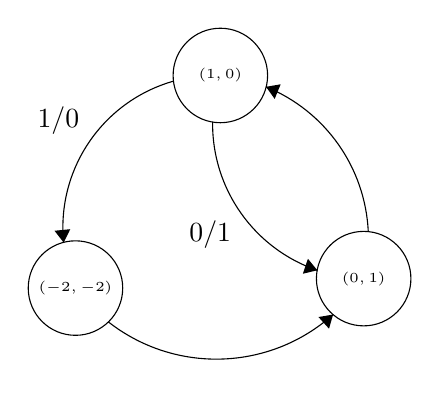
\begin{tikzpicture}[scale=0.2]
  \tikzstyle{every node}+=[inner sep=0pt]
  \draw [black] (26.6,-12.1) circle (3);
    \draw (26.6,-12.1) node {\tiny $(1,0)$};
  \draw [black] (17.4,-25.6) circle (3);
    \draw (17.4,-25.6) node {\tiny $(-2,-2)$};
  \draw [black] (35.7,-25) circle (3);
    \draw (35.7,-25) node {\tiny $(0,1)$};
  \draw [black] (16.648,-22.708) arc (-174.31762:-254.2298:9.658);
  \fill [black] (16.65,-22.71) -- (17.07,-21.86) -- (16.07,-21.96);
  \draw (17.67,-14.97) node [left] {$1/0$};
  \draw [black] (33.761,-27.277) arc (-48.14861:-128.09563:11.117);
  \fill [black] (33.76,-27.28) -- (32.83,-27.44) -- (33.5,-28.18);
  \draw [black] (29.501,-12.822) arc (67.8011:2.5992:10.451);
  \fill [black] (29.5,-12.82) -- (30.05,-13.59) -- (30.43,-12.66);
  \draw [black] (32.758,-24.474) arc (-108.88288:-180.71682:9.832);
  \fill [black] (32.76,-24.47) -- (32.16,-23.74) -- (31.84,-24.69);
  \draw (27.31,-22.21) node [left] {$0/1$};
  \end{tikzpicture}
  \end{center}
\end{frame}

\begin{frame}
  \begin{itemize}
    \item It is natural to ask for what matrices $\Am$ and vectors $\e$
      can we find a given $\A$ in $\C$, and at what vectors $\v$ are its 
      states?
    \pause
    \item It can be shown that only one $\Am$ works
    \pause
    \item Becker even found a way of computing $\Am$ given the automaton
    \pause
    \item It can also be shown that for any $\e$, if $\A$ is a subautomaton,
      its location in the structure is unique
    \pause
    \item There are infinitely many choices of $\e$ though, 
      and the goal is to understand them.
  \end{itemize}
\end{frame}

\section{Extensions}
\begin{frame}{$\Z[x]$-module}
  \begin{itemize}
    \item We can multiply vectors $\v \in \Z^m$ by scalars in $\Z$
    \pause
    \item Seemingly weird idea:
    \pause
    \begin{itemize}
      \item Can we take \emph{polynomials} as our scalars instead?
    \end{itemize}
    \pause
    \item Typically this is done by setting $x \v = \Am \v$ for some 
      linear transformation.
    \pause
    \item If only we had a obvious linear transformation floating around our
      structure that one might try\ldots
    \pause
    \item For technical reasons, we'll use $\Am^{-1}$ instead of $\Am$.
  \end{itemize}
  \pause
  \begin{defn}
    For $p \in \Z[x]$ and $\v \in \C$, put $p \cdot \v = (p(\Am^{-1}))\v$
  \end{defn}
\end{frame}

\begin{frame}
  \begin{itemize}
    \item Why should we care?
  \end{itemize}
  \pause
  \begin{thm}
    for each $\v \in \Z^m$, there is $p_{\v} \in \Z[x]$ such that 
    $p_{\v} \cdot e_1 = \v$
  \end{thm}
  \pause
  \begin{thm}
    If $\e$ is an odd vector, then 
    $\varphi_{\e} : \mathfrak{C}(\Am,\e_1) \hookrightarrow \C$ by
    $\varphi_{\e} (\v) = p_{\e} \cdot \v$ is an embedding, and preserves the 
    group structure and the residuation structure.
  \end{thm}
  \pause
  \begin{itemize}
    \item This embedding is surjective if and only if $p_{\e}$ is a unit
      in $\Z[x]/\chi$, where $\chi$ is the characteristic polynomial of $\Am^{-1}$
    \pause
    \item So different residuation vectors give groups which \emph{extend} 
      the group $\mathfrak{C}(\Am,\e_1)$
    \pause
    \item Also, if $p_{\e}$ divides $p_{\r}$, then $\mathfrak{C}(\Am,\r)$
      extends $\mathfrak{C}(\Am,\e)$.
  \end{itemize}
\end{frame}

\begin{frame}
  \begin{thm}
    If $\A$ is an automaton whose group is $\Z^m$, then for each odd state
    in $\A$, there is exactly one $\e$ which locates that state at $\e_1$
    in $\C$. Further, if $\e$ and $\r$ are two such residuation vectors,
    they differ by a unit. This procedure is effective.
  \end{thm}

  \begin{thm}
    If $\A$ has a state located at $\v \in \C$, then $\v$ is located
    at $p \cdot \v \in \mathfrak{C}(\Am, p \cdot \e)$
  \end{thm}

  \begin{itemize}
    \item Incredibly, we now understand residuation vectors!
    \pause
    \item First find $\r$ such that $\A$ has a state at $\e_1$.
    \item $\A$ is a subautomaton of $\C$ if and only if $p_{\r}$
      divides $p_{\e}$
    \item Also, if $\A$ \emph{is} a subautomaton, then 
      $q p_{\r} = p_{\e}$, and $\A$ is located at $q \cdot \e_1$
  \end{itemize}
\end{frame}

\begin{frame}
  \begin{itemize}
    \item It turns out we can ``scale by an infinite polynomial'' to
      get a universal structure which contains \emph{every} automaton
      (with the correct matrix $\Am$) at exactly one location.
    \item The construction is a bit involved, so we don't have time to
      discuss it, but it is computable, and removes the need for the
      extra parameter $\e$.
  \end{itemize}
\end{frame}

\begin{frame}{Questions?}
\end{frame}

\end{document}
